% !TeX root = ../libro.tex
% !TeX encoding = utf8

\chapter{Implementación y pruebas}

\section*{Tipo de shader para el teselado}
En esta sección se justificará el uso del tesellation shader para el estudio del teselado de una superficie.
 
\subsection*{Geometry shader}
	La ventaja de este tipo de shader es que es muy flexible a la hora de generar nuevas primitivas, ya que permite añadir primitivas totalmente disconexas.\\
	\\ En primer lugar opté por describir de forma explícita un cierto número de niveles de la función recursiva deseada, $3$ niveles concretamente. Los resultados eran aceptables pero se podía exceder el límite de vértices, quedando así una superficie incompleta. Además, el tiempo de compilación crecía de forma exponencial a medida que se añadían más niveles (para $2$ niveles era de $10$-$15$s y para $3$ no concluía).\\
	\\ Puesto que este método era costoso temporalmente y tenía muchas limitaciones, decidí implementar un algoritmo similar pero en un bucle, cuyo esquema es el siguiente:
	\begin{enumerate}
		\item Dado un lado, dividirlo en tantos segmentos como sea necesario, atendiendo a una cierta medida. Dicha medida sólo depende de las características del lado, para que el pegado sea el correcto con los triángulos adyacentes.
		\item Se realiza una división hacia el baricentro, de forma similar al punto anterior.
		\item Con los vértices de los dos puntos anteriores se genera una malla, es decir, para cada lado, se genera otro lado paralelo para cada subdivisión hacia el baricentro, manteniendo proporcionalmente las subdivisiones del lado original.
		\item Se genera una tira de triángulos cuyos vértices sean los de la malla anterior.
	\end{enumerate}
	
	Con este método los problemas anteriores se solventan en gran medida, pero dicho algoritmo es semejante al del Tessellation shader, por lo que era natural estudiar el funcionamiento en tal shader.\\
	\\ Finalmente, los inconvenientes observados han sido los siguientes:
	\begin{itemize}
		\item El número de vértices de salida está limitado por una constante predefinida, con valor GL$\_$MAX$\_$GEOMETRY$\_$OUTPUT$\_$VERTICES=$256$ (depende del hardware), es decir, como mucho se puede devolver una tira de $254$ triángulos, independientemente del tamaño del triángulo original.
		\item El shader tarda en compilarse de media entre $3$ y $5$ segundos.
	\end{itemize}
	
\subsection*{Tessellation shader}

	Este shader tiene un pequeño problema y es que la subdivisión está predefinida (equal, fractional$\_$odd o fractional$\_$even spacing), por lo que los vértices generados en la fase de control del Tessellation shader tienen un esquema fijo, para un número de subdivisiones dado. No es un gran inconveniente puesto que en la fase de evaluación se pueden variar libremente dichos vértices, siempre que se haga con cuidado (en esta fase los vértices se generan mediante coordenadas baricéntricas). \\
	\\Además, la versión de OpenGL necesaria es superior al del Geometry shader ($4.0$ frente a $3.2$).
	\\ Las ventajas con respecto al Geometry shader son las siguientes:
	\begin{itemize}
		\item El shader tarda en compilarse de media menos de $1s$.
		\item El número de vértices de salida no está tan limitado (GL$\_$MAX$\_$PATCH$\_$VERTICES$=36477$ frente a $256$).
		\item Está pensado para realizar directamente el algoritmo de teselación, por lo que no hay que implementarlo.
	\end{itemize}
	
	Al tener implementado el algoritmo de teselación, el estudio se reduce a encontrar una medida que nos indique cómo de buena es la representación de la superficie. Como la teselación de un triángulo se indica por cada lado (outer tessellation factor) y en el interior (inner tessellation), para cada tipo de medida hay que proporcionar una adicional para los lados, para que la teselación sólo dependa de lo que sucede en ellos y de esta forma pegue correctamente con el triángulo adyacente. Dicho estudio ya se ha realizado en el apartado \textbf{Estudio de la teselación}, que es el capítulo $5$ de la parte II.

\section*{Optimización del código GLSL}
	Puesto que queremos que el programa renderice la escena en tiempo real, es necesario simplificar todo lo posible el código de los shaders, sobre todo del fragment shader (se va a ejecutar para cada vértice generado en el teselado). Para ello se han tenido en cuenta los siguientes hechos (obtenidos principalmente de la Wiki de Khronos \cite{KhronosWiki}, en la sección GLSL Optimizations):
	\begin{itemize}
		\item Evitar el uso de saltos condicionales y de bucles. En caso de ser necesario algún bucle, usar los de la forma ``for(int i=$0$; i<n; i++)'' con $n$ entero constante, para permitir el desenrollado del bucle por el compilador.
		\item Utilizar ``Swizzle'' en vez de asignar vectores componente a componente.
		\item Utilizar ``MAD'', es decir, usar siempre que sea posible la multiplicación por el inverso en vez de la división (para aquellos valores ``uniform'' o constantes) y desarrollar las expresiones como una sumatoria de productos. Por ejemplo, utilizar $a*0.5 + b*0.5$ en vez de $(a+b)/2$.
		\item Utilizar ``dot'' para agrupar varias expresiones en una. De igual forma utilizar todo el cálculo vectorial y matricial posible para resumir las operaciones.
		\item Si una expresión es común para un mismo frame, calcularlo en la CPU y asignarlo como otro ``uniform'' para quitarle carga a la GPU, ya que se ejecutaría para cada primitiva o vértice (dependiendo de en qué shader se realize el cálculo).
	\end{itemize}
	
	Es cierto que el compilador ya realiza de manera automática algunas de estas optimizaciones, pero su puesta en práctica puede reducir ligeramente el tiempo de compilación.

\section*{Procesador}
Para dicho programa se ha implementado el análisis léxico usando un generador de analizadores de léxico tipo 'lex' (flex), a partir de las expresiones regulares que definen los tokens del lenguaje. También se ha implementado un analizador sintáctico LALR mediante un generador de analizadores sintácticos tipo 'yacc' (Bison), partiendo de la gramática del lenguaje, junto con las acciones semánticas que comprueban dichos errores (los errores semánticos) y generan los árboles de expresión.\\
\\Las expresiones regulares, la tabla de tokens y la gramática se han definido a partir de la especificiación BNF, ya citada en el desarrollo del proyecto (parte II, capítulo Procesador).
\\La implementación del ``procesador'' no se ha realizado desde cero, es decir, se ha partido de una implementación parcial que se aportaba en la asignatura de Procesadores de lenguajes. Dicha implementación, tras ser adaptada, sólo realizaba la traducción directa del código de entrada, junto con la comprobación de errores (léxicos, sintácticos y semánticos). La parte restante corresponde con la generación del árbol de expresión y calcular los árboles derivados, además de adecuar la salida correctamente para que se pueda utilizar como parte de un shader.\\

\section*{Visualizador}
En un principio se propuso utilizar como código de partida el proporcionado en la asignatura de Informática Gráfica, pero se observó que tenía muchas funcionalidades que no se llegarían a utilizar y cuya adaptación requeriría más tiempo. Por ello se decidió empezar de cero, pero utilizando como ``esqueleto'' un código de ejemplo de la referencia Learn OpenGL \cite{LearnOGL}, que aportaba simplemente la visualización de un objeto en una escena $3$D con una fuente de luz y una cámara sencilla.

\section*{Interfaz}
Para la implementación de la interfaz se ha utilizado la librería de código libre ``Dear ImGui'' \cite{DearImGui}, junto los complementos ``ImGui Quat'' \cite{LVector} para visualizar el vector de luz y modificarlo, e ``ImGui Dialog'' \cite{Dialog} para mostrar un diálogo con un explorador de archivos y así poder seleccionar la parametrización deseada.

\section*{Generación de informes}
Para conocer el rendimiento de la aplicación se han medido los fotogramas generados por segundo y las primitivas que hay presentes en la escena, incluyendo las que son producto del teselado.\\
\\La medición del nº de primitivas se ha realizado mediante el uso de la estructura "query" de OpenGL, la cual se actualiza cada vez que renderiza la escena. El nº de fotogramas por segundo se ha calculado manualmente, contando los fotogramas generados en cada segundo.\\
\\Además, para mayor comodidad se ha añadido una opción para realizar dichas mediciones de forma automática y escribir los resultados en un archivo cuyo nombre dependerá de la parametrización actual y el modo de visualización. Por defecto realiza $22$ medidas ($22$ segundos). Es ligeramente mayor que $20$ para después quitar la primera y/o última medida, ya que están influenciadas por la interacción del usuario con la interfaz.\\
\\Estas medidas son suficientes para observar si la aplicación está aprovechando correctamente los recursos para obtener una buena visualización de la superficie, ya que el objetivo es que funcione en tiempo real ofreciendo la mínima carga posible al sistema.

\section*{Resultados}
	En esta sección se mostrarán los datos medidos en la aplicación para comparar las técnicas usadas. Se han seleccionado 2 superficies de las disponibles como ejemplos, ``gaussiana.in'' y ``waves.in''. Los parámetros se han elegido de manera que la visualización sea similar entre los distintos modos de renderizado, minimizando el nº de triángulos de la escena para cada modo, que es el objetivo de estudio: ofrecer un nivel de aproximación específico, maximizando el rendimiento.
		
	\begin{center}
	\begin{tabular}{ | p{2cm} | | p{2cm} | p{2cm} | p{2cm} | p{2cm} | p{2cm} | }
		\hline
		\multicolumn{6}{ | c | } {gaussiana.in}\\
		\hline
		$ $ &
		\multicolumn{5}{ | c | } {FPS}\\
		\hline
		Modo & Min & Max & Media & Mejora (fps) & Mejora ($\%$) \\
		\hline
		No tess.    & $205$ & $250$ & $231,54$ & $-$ & $-$ \\
		Normal tess.    & $253$ & $278$ & $267,63$ & $+36,09$ & $+15,58$ \\
		Improve1 & $242$ & $282$ & $266,63$ & $+35,09$ & $+15,15$ \\
		Improve2 & $\boldsymbol{255}$ & $\boldsymbol{284}$ & $\boldsymbol{273,72}$ & $\boldsymbol{+42.18}$ & $\boldsymbol{+18,21}$ \\
		\hline
		$ $ &
		\multicolumn{5}{ | c | } {Triángulos}\\
		\hline
		Modo & Min & Max & Media & Mejora (tri.) & Mejora ($\%$) \\
		\hline
		No tess.    & $20000$ & $20000$ & $20000,00$ & $-$ & $-$ \\
		Normal tess.    & $10547$ & $11802$ & $11165,5$ & $-8834,50$ & $-44,17$ \\
		Improve1 & $8267$ & $10232$ & $9100,00$ & $-10900,00$ & $-54,5$ \\
		Improve2 & $\boldsymbol{6642}$ & $\boldsymbol{10120}$ & $\boldsymbol{8212,68}$ & $\boldsymbol{-11787,31}$ & $\boldsymbol{-58,93}$ \\
		\hline
	\end{tabular}
	\end{center}
	\begin{figure}[h]
  		\centering
  		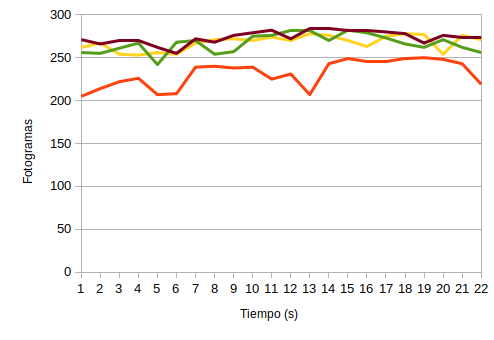
\includegraphics[width=0.435\textwidth]{performance/diagrama_gauss_fps_rec}
  		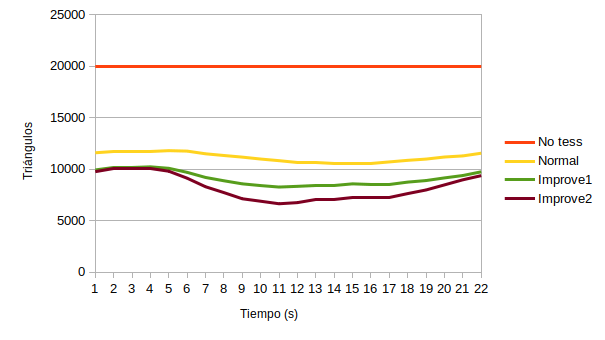
\includegraphics[width=0.555\textwidth]{performance/diagrama_gauss_triangulos}
  		\caption{Gráfica de la animación de rotación en gauss.in}
  		\label{fig:diagramas_gauss}
	\end{figure}
	
	\newpage
	\begin{center}
	\begin{tabular}{ | p{2cm} | | p{2cm} | p{2cm} | p{2cm} | p{2cm} | p{2cm} | }
		\hline
		\multicolumn{6}{ | c | } {waves.in}\\
		\hline
		$ $ &
		\multicolumn{5}{ | c | } {FPS}\\
		\hline
		Modo & Min & Max & Media & Mejora (fps) & Mejora ($\%$) \\
		\hline
		No tess.    & $21$ & $24$ & $21,81$ & $-$ & $-$ \\
		Normal tess. & $53$ & $63$ & $58,27$ & $+36,45$ & $+167,08$ \\
		Improve1 & $\boldsymbol{63}$ & $72$ & $64,68$ & $+42,86$ & $+196,45$ \\
		Improve2 & $62$ & $\boldsymbol{87}$ & $\boldsymbol{69,86}$ & $\boldsymbol{+48.04}$ & $\boldsymbol{+220,20}$ \\
		\hline
		$ $ &
		\multicolumn{5}{ | c | } {Triángulos}\\
		\hline
		Modo & Min & Max & Media & Mejora (tri.) & Mejora ($\%$) \\
		\hline
		No tess.    & $1000000$ & $1000000$ & $1000000,00$ & $-$ & $-$ \\
		Normal tess.    & $456480$ & $637537$ & $550527,77$ & $-449472,22$ & $-44,94$ \\
		Improve1 & $197244$ & $224222$ & $212327,00$ & $-787673,00$ & $-78,76$ \\
		Improve2 & $\boldsymbol{194703}$ & $\boldsymbol{223824}$ & $\boldsymbol{210390,31}$ & $\boldsymbol{-789609,68}$ & $\boldsymbol{-78,96}$ \\
		\hline
	\end{tabular}
	\end{center}
	\begin{figure}[h]
  		\centering
  		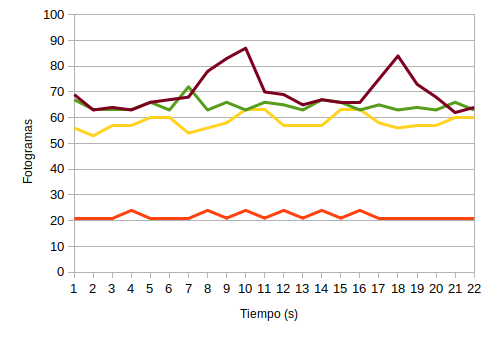
\includegraphics[width=0.435\textwidth]{performance/diagrama_waves_fps_rec}
  		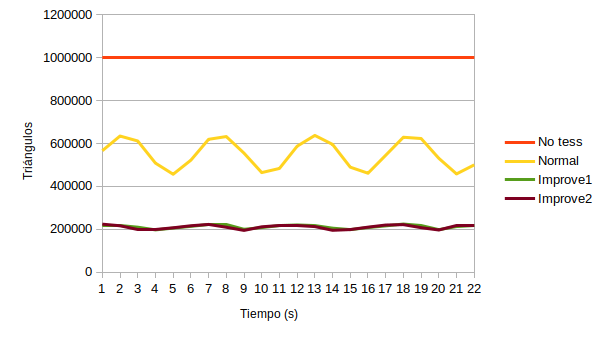
\includegraphics[width=0.555\textwidth]{performance/diagrama_waves_triangulos}
  		\caption{Gráfica de la animación de rotación en waves.in}
  		\label{fig:diagramas_waves}
	\end{figure}
	
	
	\newpage
	Las siguientes imágenes corresponden con la parametrización ``gaussiana.in'' con los distintos modos de visualización, donde para cada modo se ha buscado la configuración óptima, es decir, aquella en la que se ve visualmente bien y el nº de triángulos es mínimo. Por tanto, las $4$ imágenes debería ser exactamente iguales en modo relleno, en modo malla se verán las distintas distribuciones de triángulos subyacentes:
	\begin{figure}[h]
		\begin{minipage}{0.48\textwidth}
  			\centering
  			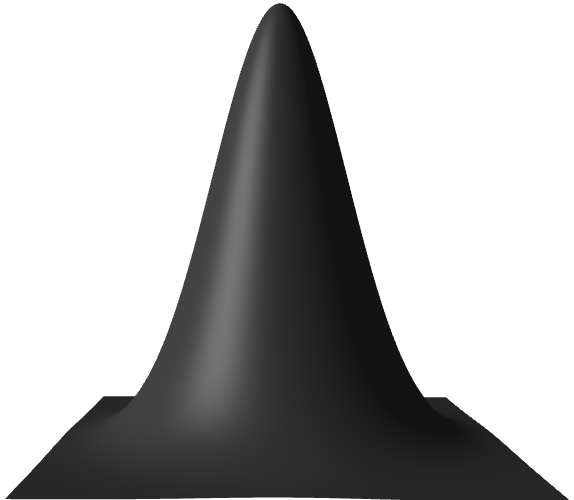
\includegraphics[width=0.9\textwidth]{performance/gauss_notess}
  			\caption{gaussiana.in sin teselar}
		\end{minipage}\hfill
		\begin{minipage}{0.48\textwidth}
  			\centering
  			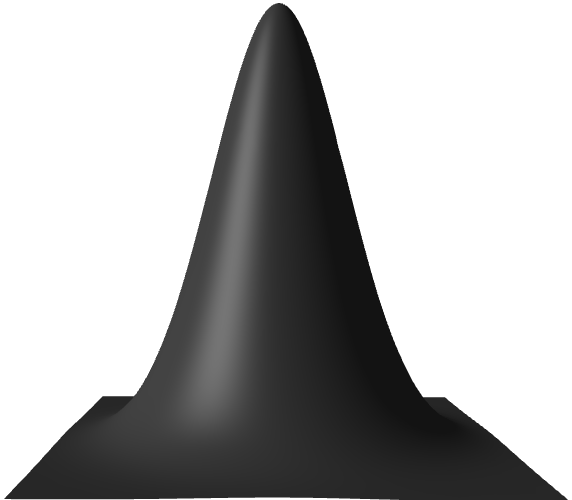
\includegraphics[width=0.9\textwidth]{performance/gauss_tessbad}
  			\caption{gaussiana.in teselado normal}
		\end{minipage}\hfill
		
		\begin{minipage}{0.48\textwidth}
  			\centering
  			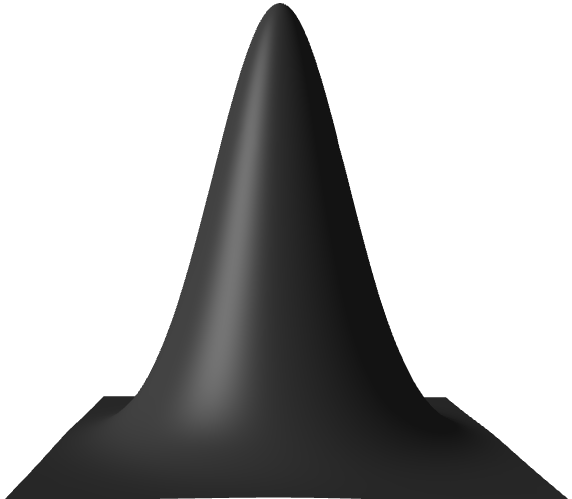
\includegraphics[width=0.9\textwidth]{performance/gauss_improve1}
  			\caption{gaussiana.in improve$1$}
		\end{minipage}\hfill
		\begin{minipage}{0.48\textwidth}
  			\centering
  			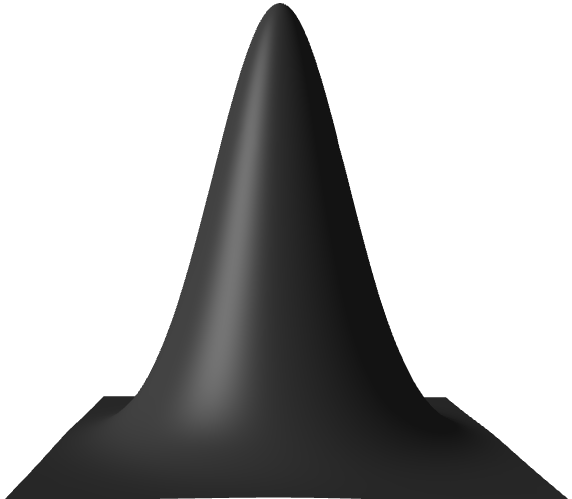
\includegraphics[width=0.9\textwidth]{performance/gauss_improve2}
  			\caption{gaussiana.in improve$2$}
		\end{minipage}\hfill
  		\label{fig:imagenes_gauss}
	\end{figure}	
	
	\newpage
	\begin{figure}[h]
		\begin{minipage}{0.48\textwidth}
  			\centering
  			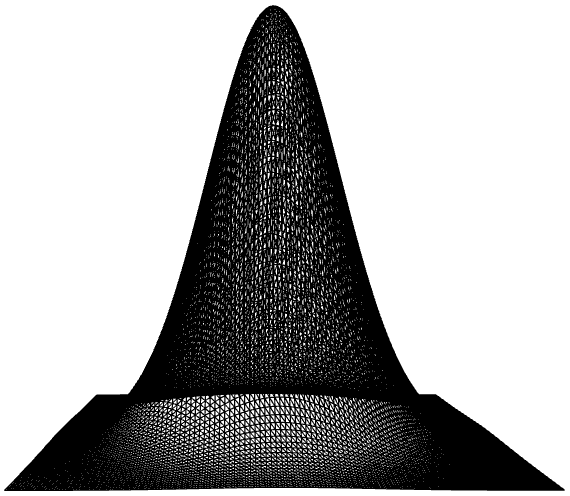
\includegraphics[width=0.9\textwidth]{performance/gauss_pol_notess}
  			\caption{gaussiana.in sin teselar}
		\end{minipage}\hfill
		\begin{minipage}{0.48\textwidth}
  			\centering
  			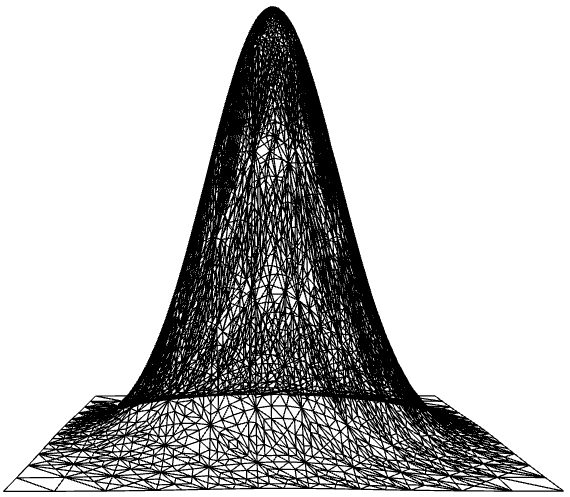
\includegraphics[width=0.9\textwidth]{performance/gauss_pol_tessbad}
  			\caption{gaussiana.in teselado normal}
		\end{minipage}\hfill
		
		\begin{minipage}{0.48\textwidth}
  			\centering
  			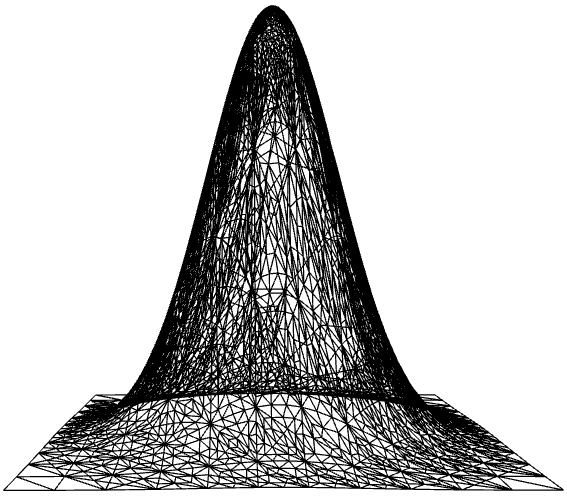
\includegraphics[width=0.9\textwidth]{performance/gauss_pol_improve1}
  			\caption{gaussiana.in improve$1$}
		\end{minipage}\hfill
		\begin{minipage}{0.48\textwidth}
  			\centering
  			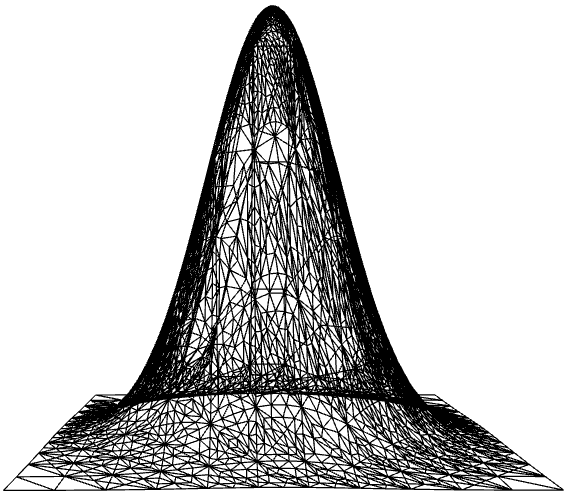
\includegraphics[width=0.9\textwidth]{performance/gauss_pol_improve2}
  			\caption{gaussiana.in improve$2$}
		\end{minipage}\hfill
  		\label{fig:imagenes_gauss_pol}
	\end{figure}	
	
	Seguidamente se muestran las imagenes correspondientes a la parametrización ``waves.in''. Sin embargo, debido a la complejidad de la superficie base (plano horizontal perturbado con un coseno), para el modo ``sin teselado'' es imposible llegar a una buena representación incluso utilizando una malla inicial de $1$ millón de triángulos, debido a la aparición de efectos ópticos, por la uniformidad de la malla inicial (parece haber más de un foco mientras que sólo hay uno).\\
	\\También es posible observar que al pasar de ``improve$1$'' a ``improve$2$'' puede aparecer algún segmento sin teselar. Se debe a que detecta que es un segmento oculto, mediante un cálculo basado en los extremos del segmento, pero como ya se comentó anteriormente esta funcionalidad está pensada para superficies específicas.
	\newpage
	\begin{figure}[h]
  		\centering
  		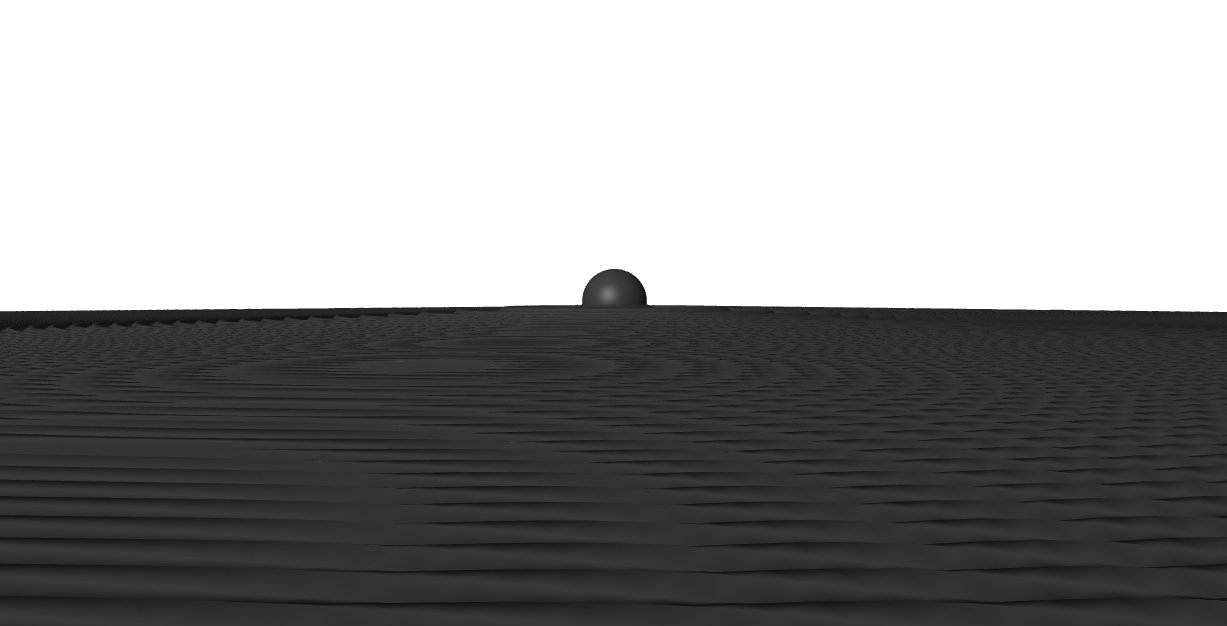
\includegraphics[width=0.9\textwidth]{performance/waves_notess}
  		\caption{waves.in sin teselar}
  		\vspace{0.5cm}
  		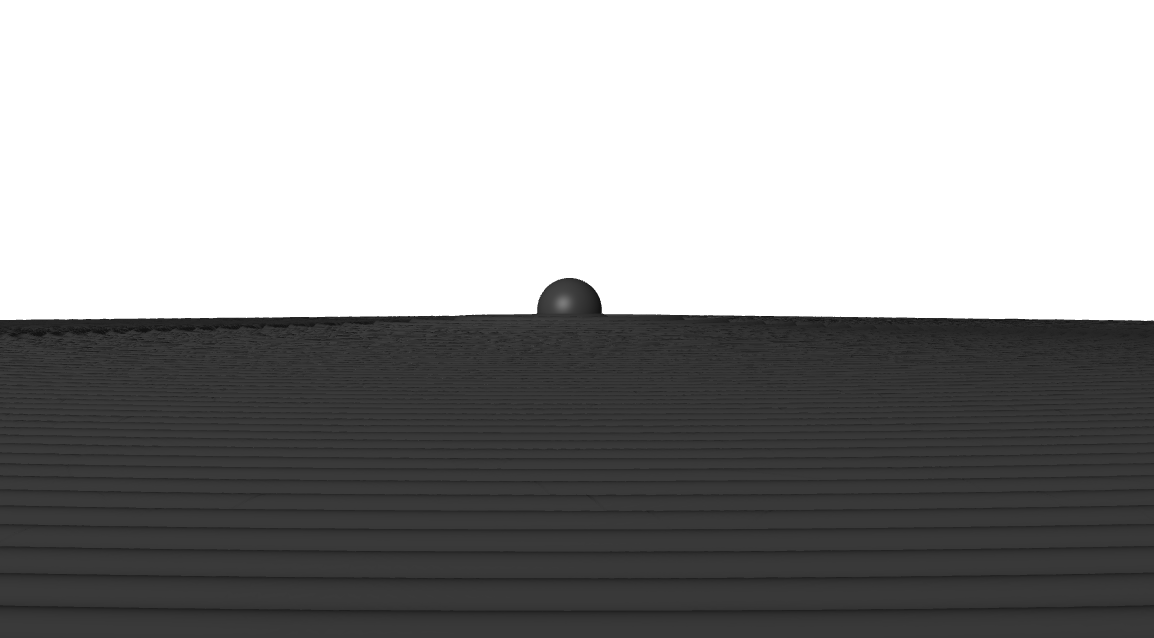
\includegraphics[width=0.9\textwidth]{performance/waves_tessbad}
  		\caption{waves.in teselado normal}
  		\vspace{0.5cm}
  		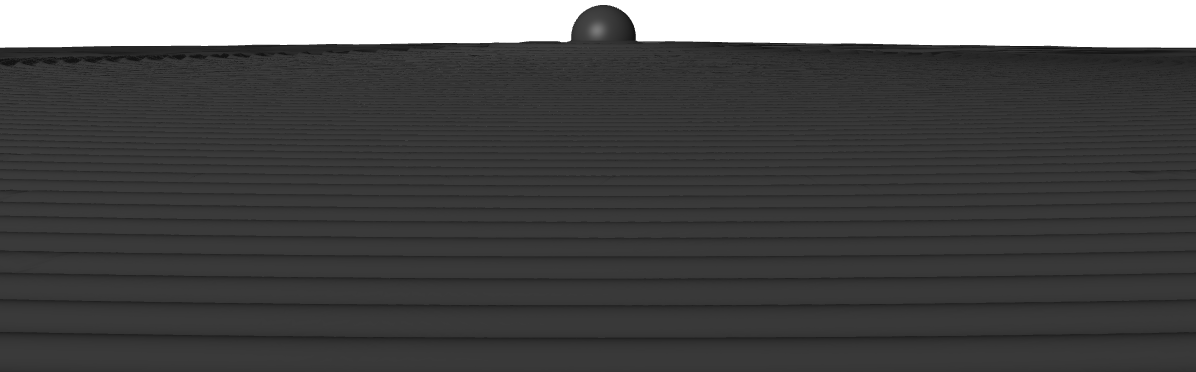
\includegraphics[width=0.9\textwidth]{performance/waves_improve1}
  		\caption{waves.in improve$1$}
  		\vspace{0.5cm}
  		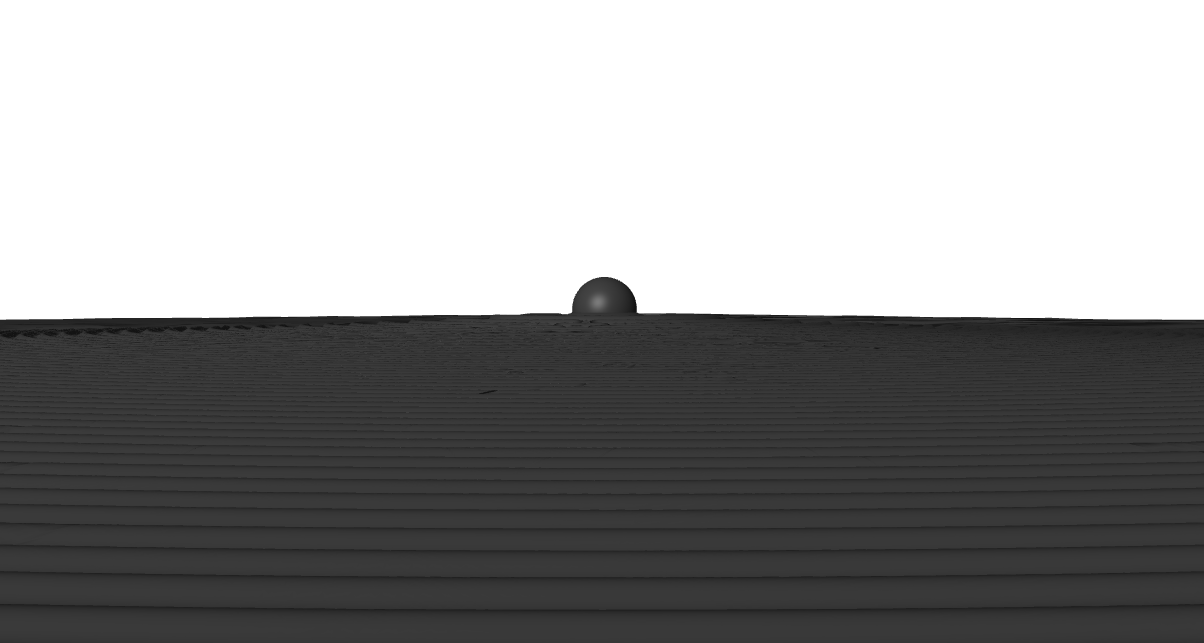
\includegraphics[width=0.9\textwidth]{performance/waves_improve2}
  		\caption{waves.in improve$2$}
  		\label{fig:imagenes_waves}
	\end{figure}	
	\begin{figure}[h]
  		\centering
  		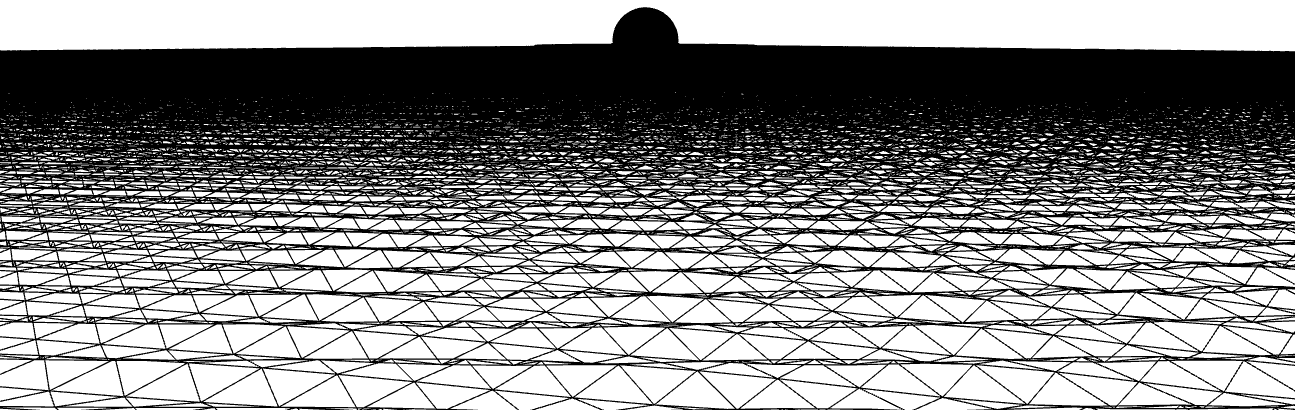
\includegraphics[width=0.9\textwidth]{performance/waves_pol_notess}
  		\caption{waves.in sin teselar}
  		\vspace{0.5cm}
  		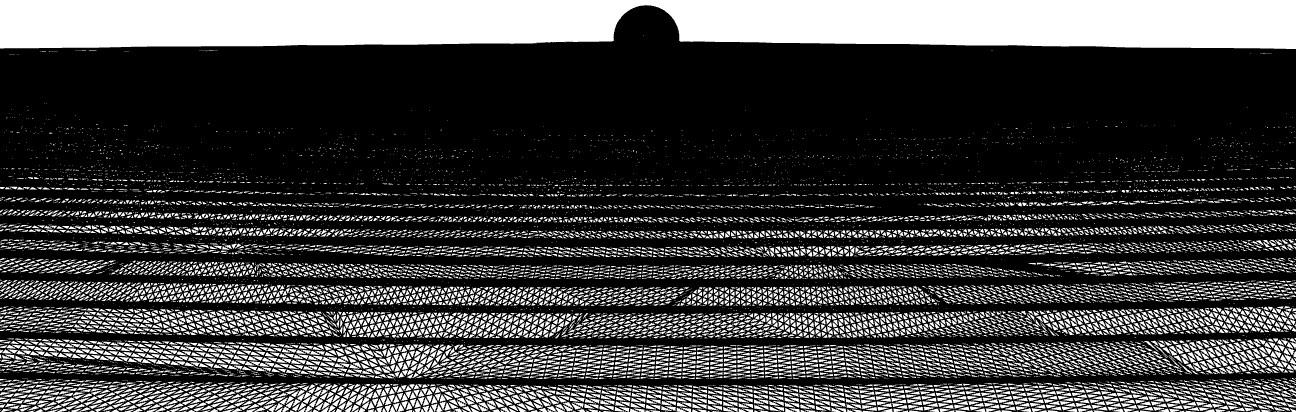
\includegraphics[width=0.9\textwidth]{performance/waves_pol_tessbad}
  		\caption{waves.in teselado normal}
  		\vspace{0.5cm}
  		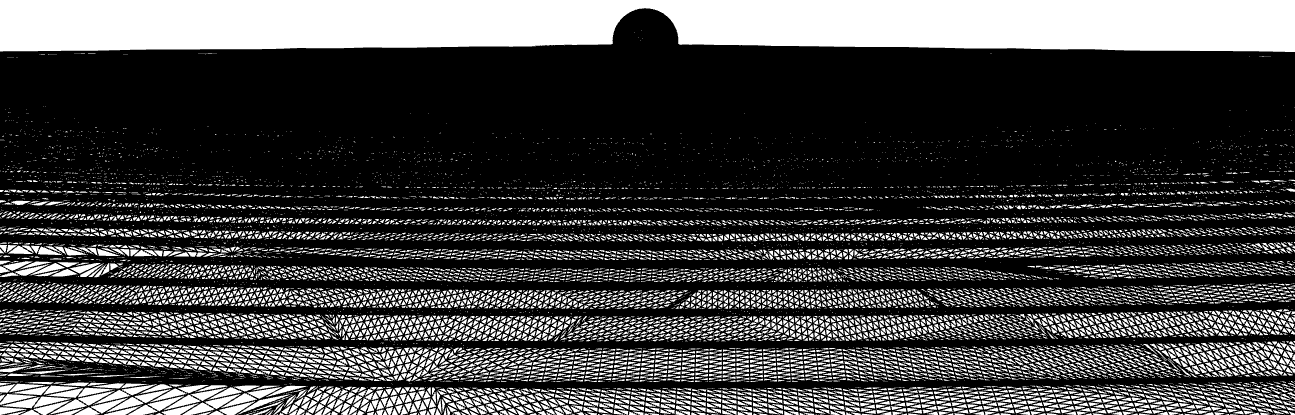
\includegraphics[width=0.9\textwidth]{performance/waves_pol_improve1}
  		\caption{waves.in improve$1$}
  		\vspace{0.5cm}
  		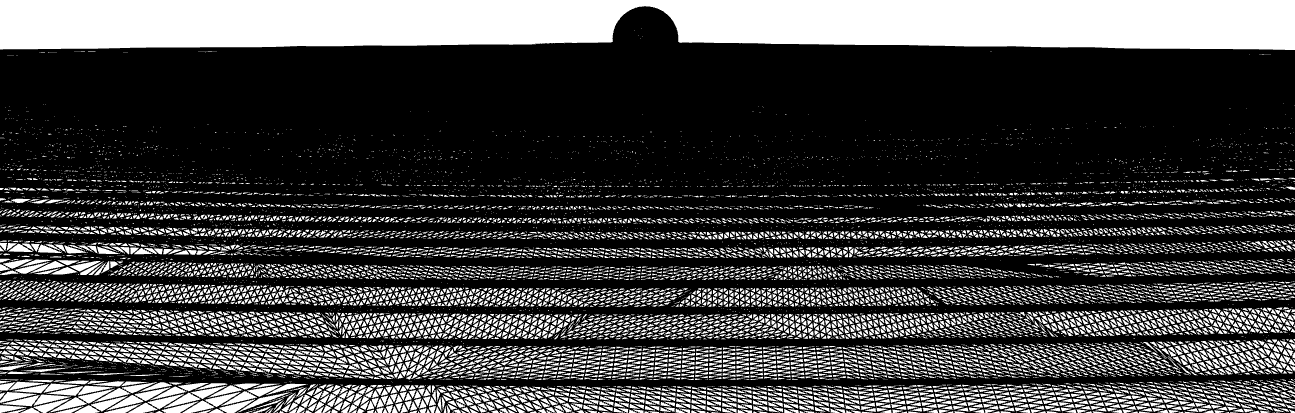
\includegraphics[width=0.9\textwidth]{performance/waves_pol_improve2}
  		\caption{waves.in improve$2$}
  		\label{fig:imagenes_waves_pol}
	\end{figure}	
	\newpage
		
		
\endinput
%------------------------------------------------------------------------------------
% FIN DEL CAPÍTULO. 
%------------------------------------------------------------------------------------
